\documentclass{article}
\usepackage{graphicx}
\begin{document}
	\section{Logic Gate}
	Logic gates perform logical operations that take binary input (0s and 1s) and produce  a single binary output. They are used in most electronic device including:
	\begin{table}[h!]
		\begin{center}
			\caption{LOGIC GATES}
	 		\label{tab:table1}
			\begin{tabular}{|l|c|c|}
				\hline
				Smartphones
				&
				Tablets
				&
				Memory Devices
				\\
				\hline
				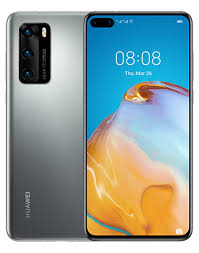
\includegraphics[width=0.2\linewidth]{smartphone1}
				&
				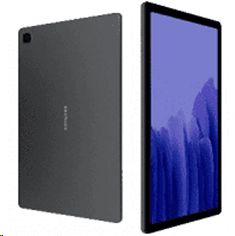
\includegraphics[width=0.25\linewidth]{Tablet}
				&
		     	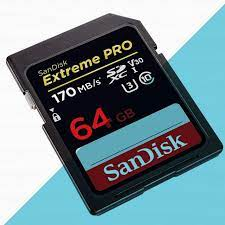
\includegraphics[width=0.1\linewidth]{memory disk}
				\\
				  \hline
				  \end{tabular}
			
				
		\end{center}
	\end{table}
	
\end{document}